\section{Results}



We present results for three major settings:
\begin{itemize}
    \item Performance of fully pre-trained large language models across different number of shots.
    \item Development of performance over the course of training on our pre-training datamix.
    \item Scaling laws ablations across different compute flops and seeds.
\end{itemize}

% \subsection{Performance on fully trained models}
\subsection{Informativeness for fully trained models}

With the goal to get an overall estimate of the difficulty of the task and the extent to which it can discriminate models, we first consider the performance of fully pre-trained models from the respective model series.
For each of the models, we compute results with variable number of shots.
We report the results in \cref{fig:shot_performance}, along with a chance baseline and the results of a fine-tuned BERT model.
For all models, we observe rather poor zero-shot performance for all tasks, except AbductiveNLI, confirming previously reported results by \citet{ohmer2024form} and \citet{weber-etal-2023-mind}, among others.
When more shots are added performance starkly improves.
Even with just one shot, the performance is significantly better than the zero shot accuracy; Adding more than three or four examples in the few shots does not improve performance much and saturates till 10 shots. 
Among the five benchmarks, the most challenging benchmark is ANLI.
Although the 70 and 405B models far outperform the finetuned BERT baseline, they do not exceed 70\% accuracy -- to some extent confirming the difficulty of the benchmark reported by \citet{brown2020language}.

In terms of discriminability, virtually all benchmarks provide a clear gap between the smaller and larger models.
For example, for the Llama series, 405B performs the best followed by 70B and then the 8B. 
Though these three models are trained on the same amount of text tokens, performance clearly improves with scale. 
The exception to this pattern is AbductiveNLI, which appears to be near-saturated already at 70B scale, at a performance of around 85\%.
We conclude, from these results, that the benchmarks under consideration provide a useful signal to compare trained-out models, though it is unclear to what extent their performance has saturated, a question that we discuss in more detail later in this paper (\cref{sec:}).

% Another important thing to observe is the performance comparison with fine-tuned BERT. 
% \citet{brown2020languagemodelsfewshotlearners} observed chance accuracies for GPT-3 models on the ANLI task. 
% Even with scale and few shot examples, the performance only improved marginally. 
% This might have been a factor in the community dropping NLI tasks as benchmarks for decoder-only models like GPT, Llama, Mistral, Gemma, etc. 
% In our study, we observe performance of more capable models like Llama 405B to be on-par or better than the fine-tuned BERT performance, even though no training data from the NLI tasks is used during the pre-training of LLMs. 
% The difference is clearly visible for ANLI and AbductiveNLI, where Llama-3.1 405B performances significantly better than fine-tuned BERT.

\begin{figure*}[t]
    \begin{subfigure}[b]{\textwidth}
        \centering
        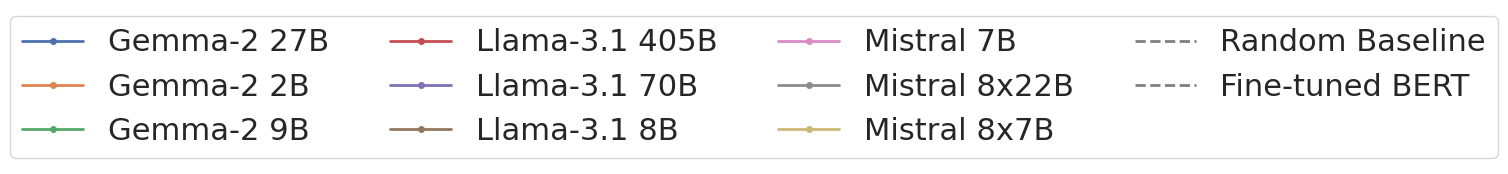
\includegraphics[width=0.8\textwidth]{figures/legend}
        \vspace{-2mm}
    \end{subfigure}\\
    \begin{subfigure}[b]{0.217\textwidth}
    \centering
    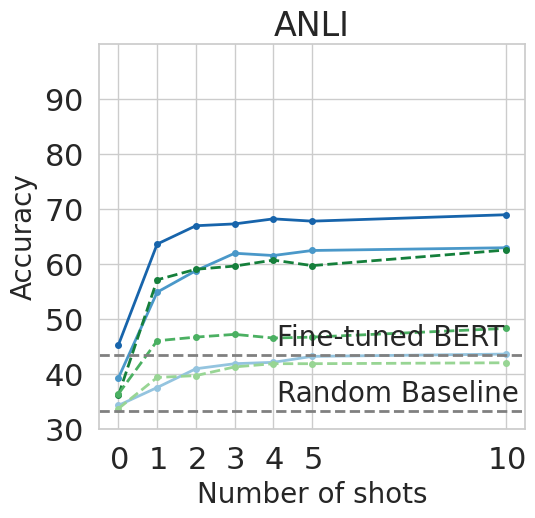
\includegraphics[height=3.2cm]{figures/anli}
    \caption{ANLI}
    \end{subfigure}
    \label{fig:anli}
    \begin{subfigure}[b]{0.19\textwidth}
    \centering
    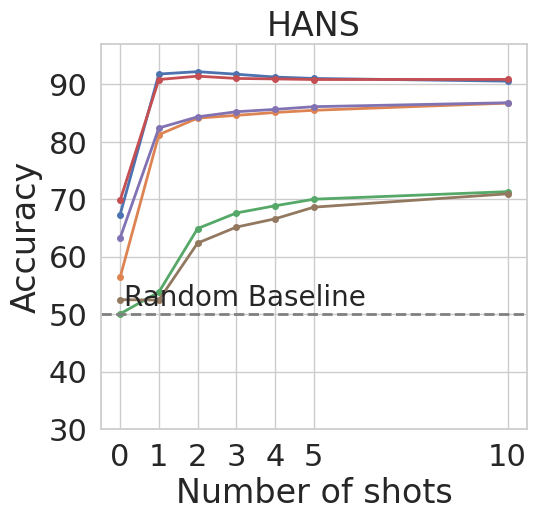
\includegraphics[height=3.2cm, trim=25mm 0 0 0, clip]{figures/hansnli}
    \caption{HansNLI}
    \label{fig:hansnli}
    \end{subfigure}
    \begin{subfigure}[b]{0.19\textwidth}
    \centering
    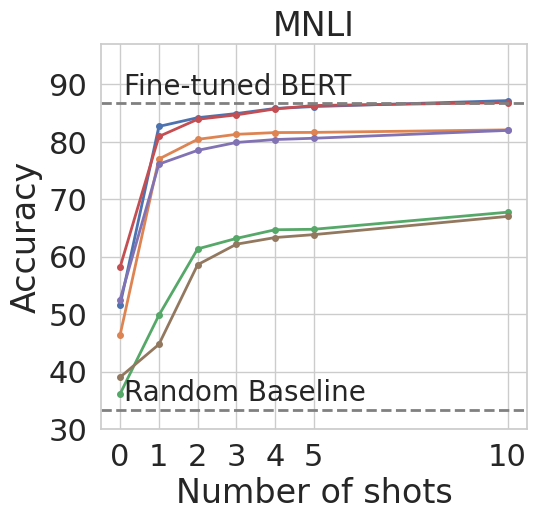
\includegraphics[height=3.2cm, trim=25mm 0 0 0, clip]{figures/mnli_matched}
    \caption{MNLI}
    \label{fig:mnli}
    \end{subfigure}
    \begin{subfigure}[b]{0.19\textwidth}
    \centering
    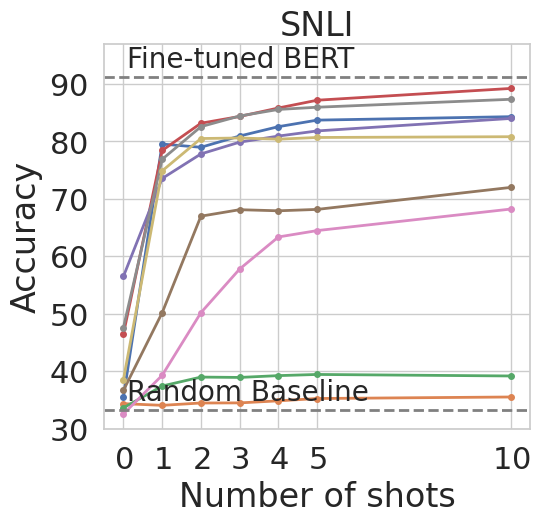
\includegraphics[height=3.2cm, trim=25mm 0 0 0, clip]{figures/snli}
    \caption{SNLI}
    \label{fig:hansnli}
    \end{subfigure}
    \begin{subfigure}[b]{0.19\textwidth}
    \centering
    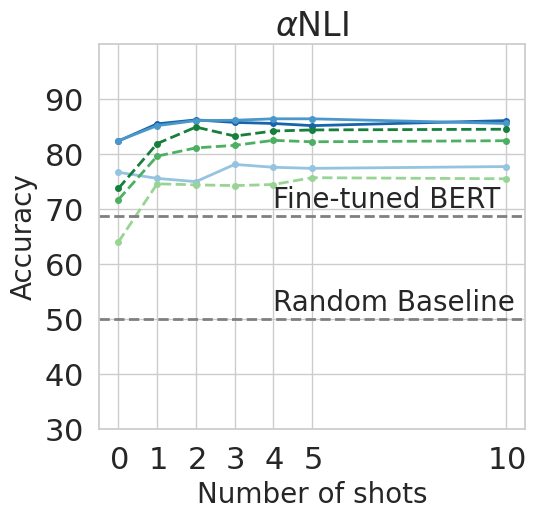
\includegraphics[height=3.2cm, trim=25mm 0 0 0, clip]{figures/abductivenli}
    \caption{AbductiveNLI}
    \label{fig:mnli}
    \end{subfigure}
    \caption{\textbf{Performance across shots.} We show performance across shots for 6 trained-out models, for ANLI, HANS, MNLI, SNLI and AbductiveNLI.}\label{fig:shot_performance}
\end{figure*}

% \subsection{Performance development over training}
\subsection{Informativeness during training}\label{subsec:during_training}

Next, we investigate whether NLI datasets may provide a good signal during training.
To this end, we pre-train Llama-3 architecture based 8B and 70B models from scratch for 2T tokens.
The details of the pre-training mix are provided in \cref{sec:appendix}. 

\paragraph{Development during training} In \cref{fig:performance_training}, we show how (four-shot) performance develops during training.
We see that for most benchmarks, the 8B and 70B model quickly start to diverge.
The 70B model starts improving after around 250B tokens, for ANLI and Abductive NLI, it crosses fine-tuned BERT performance after around 500B tokens.
On the other hand, the development of performance for the 8B model is slow, at this scale not exceeding chance accuracy for HansNLI, MNLI, and SNLI. 
From the final model performance of 8B depicted in Figure \cref{fig:shot_performance}, we can conclude that the 8B model improves fairly late during the training stage. 
We did not have the budget to do the full pre-training run, but longer training definitely seems to help on NLI tasks, further confirming the claim that NLI models can still provide a helpful signal.

\begin{figure*}[t]
    \begin{subfigure}[b]{\textwidth}
        %\centering
        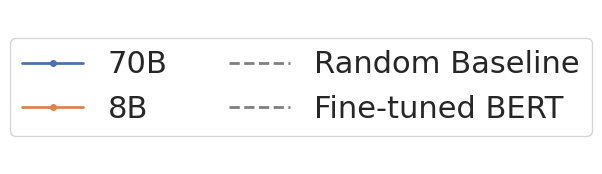
\includegraphics[width=0.3\textwidth]{figures/training_legend}
        \vspace{-2mm}
    \end{subfigure}\\
    \begin{subfigure}[b]{0.20\textwidth}
    \centering
    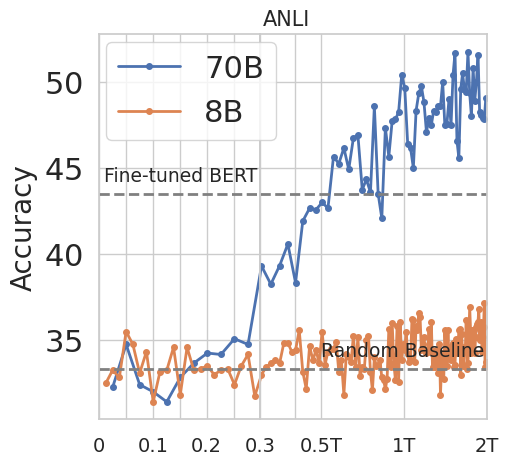
\includegraphics[height=3.2cm]{figures/anli_intermediate}
    \caption{ANLI}
    \end{subfigure}
    \label{fig:anli}
    \begin{subfigure}[b]{0.19\textwidth}
    \centering
    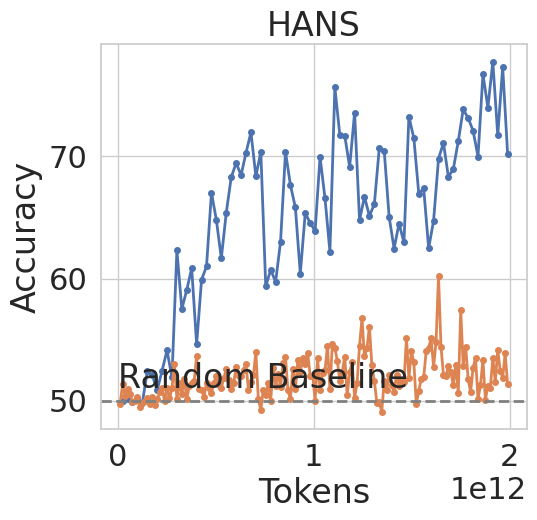
\includegraphics[height=3.2cm, trim=11mm 0 0 0, clip]{figures/hansnli_intermediate}
    \caption{HansNLI}
    \label{fig:hansnli}
    \end{subfigure}
    \begin{subfigure}[b]{0.19\textwidth}
    \centering
    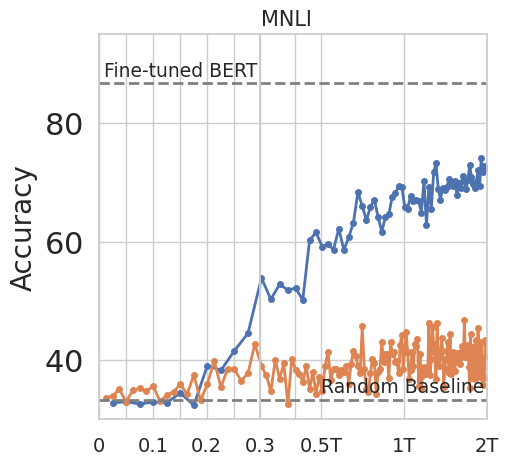
\includegraphics[height=3.2cm, trim=11mm 0 0 0, clip]{figures/mnli_matched_intermediate}
    \caption{MNLI}
    \label{fig:mnli}
    \end{subfigure}
    \begin{subfigure}[b]{0.19\textwidth}
    \centering
    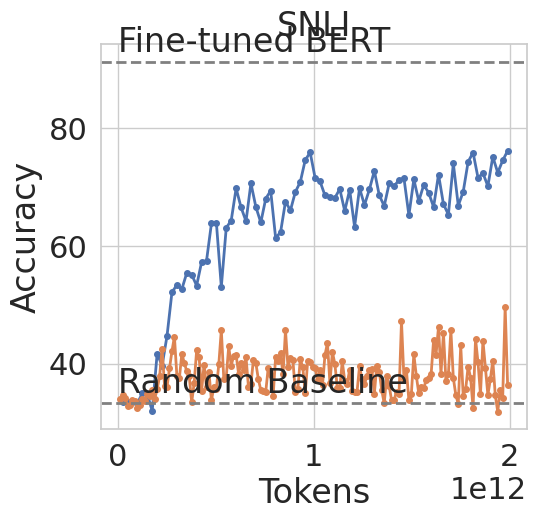
\includegraphics[height=3.2cm, trim=11mm 0 0 0, clip]{figures/snli_intermediate}
    \caption{SNLI}
    \label{fig:hansnli}
    \end{subfigure}
    \begin{subfigure}[b]{0.19\textwidth}
    \centering
    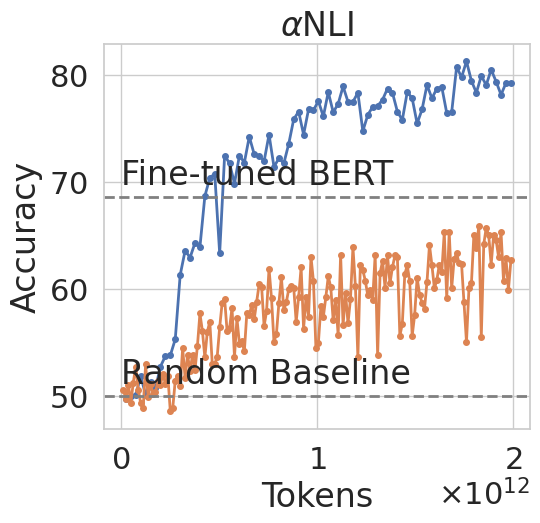
\includegraphics[height=3.2cm, trim=11mm 0 0 0, clip]{figures/abductivenli_intermediate}
    \caption{AbductiveNLI}
    \label{fig:mnli}
    \end{subfigure}
    \caption{\textbf{Performance during training.} We show how performance for the five benchmarks develops during training, for two Llama-3 style models.}\label{fig:performance_training}
\end{figure*}

\paragraph{Utility for ablations}
A requirement for a benchmark to provide a useful signal during training is that it develops relatively monotonically during training.
The plots in \cref{fig:performance_training} suggest that this is not the case for most of the benchmarks.
Following \citet{variancepaper}, we quantify the benchmarks' monotonicity on both discrete (accuracy) and continuous metrics (NLL).%
\footnote{Tracking continuous metrics like negative log likelihood (NLL) over the course of the training generally provides more monotonic results than discrete metrics such as accuracy.}
In \cref{tab:monotonicity}, we can see that, despite the benchmarks' moderate sizes, monotonicity is low for accuracy as well as NLL, suggesting that the benchmark may not be suitable for monitoring performance on small number of closely-spaced checkpoints.

\begin{table}
\centering
\resizebox{0.45\textwidth}{!}{
\begin{tabular}{lcccc}
    %\toprule
    %Model $\rightarrow$ 
    & \multicolumn{2}{c}{8B} & \multicolumn{2}{c}{70B} \\
    % \toprule
    %Benchmark $\downarrow$
    & $mon_{disc}$  & $mon_{cont}$ & $mon_{disc}$ & $mon_{cont}$ \\
    \toprule
    $\alpha$NLI & 0.62 & 0.62 & 0.79 & 0.79 \\
    \midrule
    ANLI & - & - & 0.67 & 0.47 \\
    \midrule
    HANS & 0.32 & 0.46 & 0.57 & 0.63 \\
    \midrule
    MNLI & 0.34 & 0.51 & 0.77 & 0.80 \\
    \midrule
    SNLI & 0.05 & 0.38 & 0.64 & 0.65 \\
    \bottomrule
    \end{tabular}
}
\caption{Monotonicity values for the 8B and 70B models during the course of the training. We report both the discrete ($mon_{disc}$) and continuous ($mon_{cont}$) monotonicity values.}
\label{tab:monotonicity}
\end{table}


\begin{figure*}[ht]
    \centering
    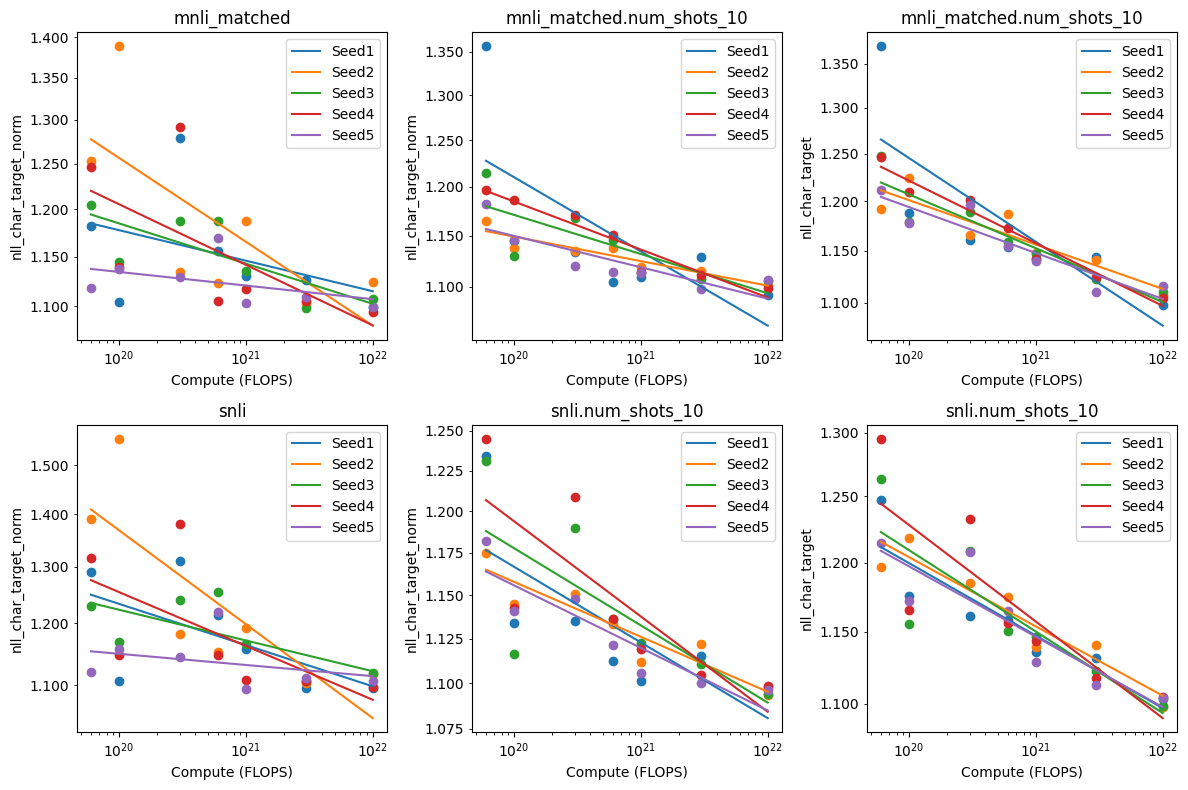
\includegraphics[width=0.95\textwidth]{nli_plots/sl_fits_mnli_snli.png}
    \caption{Scaling law curve fits across different compute FLOPs}
    \label{fig:sl_mnli_snli}
\end{figure*}

\paragraph{Q1: Does NLI provide signal for LLMs?}
We show \begin{enumerate}
    \item curves + scores on trained-out models.  Conclusion: ? Should say something about whether it is separating models in early stages of training, and whether it is monotonic, how much variance etc.
    \item Trained out model scores. Tentative conclusion (pending numbers): with the exception of abductive NLI, these datasets allow to distiguish models of different sizes. Doesn't work at all with zero-shot (which can explain some previous results?), but with one or two shots we get decent scores. ANLI seems to be the most challenging with around 70\% accuracy on the 405B model.
    \item Ablations: conclusion??
\end{enumerate}

\section{Analysis with ChaosNLI}

\citet{nie-etal-2020-learn} release the ChaosNLI dataset, which is comprised of human annotations for a subset of MNLI, SNLI, and AbductiveNLI. They collect 100 human annotations for 3113 samples for MNLI and SNLI, and 1532 samples in AbductiveNLI. In this section, we analyse the performance of models with respect to the majority labels and entropy of the label distribution according to the human annotators.

We first look at the change in accuracy when we change the ground truth labels to majority labels according to the human annotators in ChaosNLI. We only consider the 4 shot setting for this. These results are presented in Table \ref{tab:chaos_acc}. The MNLI, SNLI, and AbductiveNLI subsets in ChaosNLI are represented as ChaosNLI-M, ChaosNLI-S, and ChaosNLI-A respectively. For all three subsets, we observe an increase in model performance by changing the ground truth based on the human majority. The only exception is the 70B model for ChaosNLI-S. This represents some level of agreement between the model prediction and human preference. And the updated ground truth according to the human preferences increases the model performance.

\begin{table*}
    \centering
    \begin{tabular}{c|cc|cc|cc}
    \textbf{Benchmark} & \textbf{8B (Old)} & \textbf{8B (New)} & \textbf{70B (Old)} & \textbf{70B (New)} & \textbf{405B (Old)} & \textbf{405B (New)} \\
    \hline
    ChaosNLI-M & 49.468 & 50.969 & 57.661 & 67.542 & 64.04 & 69.669 \\
    ChaosNLI-A & 77.546 & 78.003 & 86.358 & 87.206 & 85.509 & 86.097 \\
    ChoasNLI-S & 55.284 & 55.482 & 60.436 & 58.52 & 64.597 & 67.305 \\
    \end{tabular}
\caption{Change in Accuracy for ChaosNLI when changing the ground truth to the majority label according to human annotators.}
\label{tab:chaos_acc}
\end{table*}

We look at the probability distribution according to the models over the three labels (\textit{Entailment}, \textit{Neutral}, and \textit{Contradiction}) and compute the Jensen-Shannon Divergence (JSD) \citep{menendez1997jensen} over the softmax probability distribution and human annotator distribution of the labels. Mathematically, JSD is defined as:

\begin{equation}
    \scriptstyle JSD(p || q) = \sqrt{\frac{1}{2}KL(p || m) + \frac{1}{2}KL(q || m)}
\end{equation}

where $p$ is the human annotator distribution, $q$ is the softmax probability distribution, and $m = \frac{1}{2}(p + q)$. The benefit of using JSD over KL divergence is that it is symmetric and bounded between 0 and 1.

\begin{figure*}
    \centering
    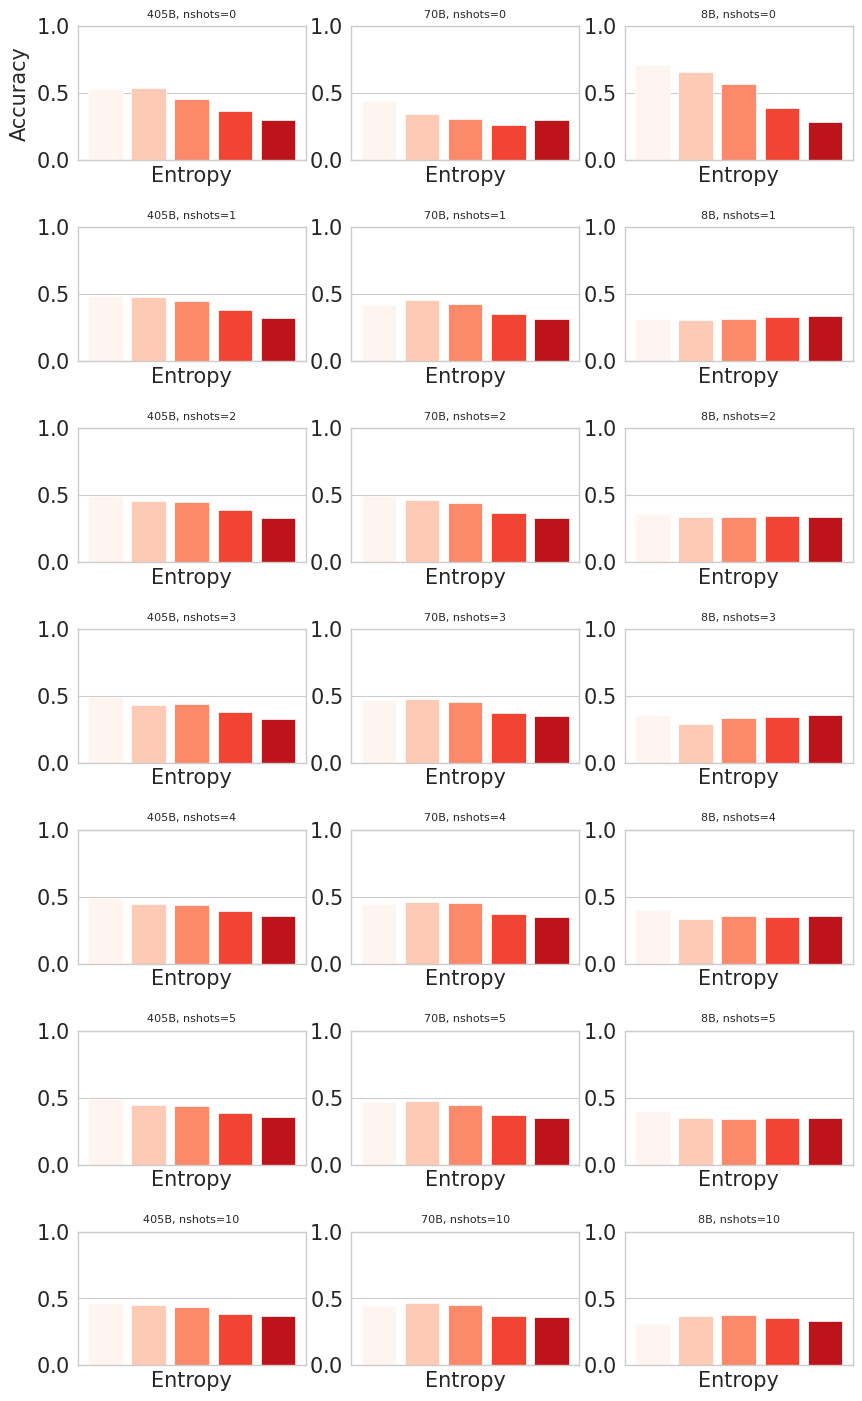
\includegraphics[width=0.98\linewidth]{nli_plots/mnli_matched_entropy_acc.png}
    \caption{Accuracy vs entropy plots for MNLI}
    \label{fig:entropy_accuracy_mnli}
\end{figure*}

NB: put contamination results somewhere.

Overall conclusion: seems to be useful both for training and trained-out models, an open question however is, is there still room to improve?

\paragraph{Q2: Is there still room for improvement?}
We do an light-weight manual analysis (e.g. check 20 examples).
Probable conclusion: there may be some errors, but oftentimes models make incorrect predictions on samples on which humans may disagree too.

To substantiate this claim, we consider chaosNLI.
We show 1) entropy plots for various models, these show that the larger models have pretty much perfect perfrmance on samples where humans agree across the board, but drop off on other examples. Smaller models don't get perfect performance also on the former. Results also show that a small amount of errors is due to annotation errors (or not matching majority labels), because the `corrected' accuracy is slightly higher than the non-corrected accuracy.
2) We show KL-divergence with human distributions. Conclusion: this gets better with scale (contradicts earlier findings!), but still far away from human alignment. Still room for improvement. We check how stable this signal is across training (so we show curves of KL/JSD and see whether this provides a astable signal.


% \begin{itemize}
%   \item Final pre-trained model result analysis. How model size, prompts, and shots affect things across various tasks.
%   \item Development of model performance for a given task across model sizes.
%   \item Correlation of model performance development with other commonsense/normal reasoning tasks (race, obqa, mmlu, math, etc.)
%   \item Results on ChaosNLI and how model scores relate to the distribution of human judgements. Model size/prompt analysis for this too.
%   \item Large models are good, but is it because of better models/training or just contamination? Contamination Analysis on various benchmarks.
%   \item Can NLI tasks help in pre-training ablations? Results on seed models and models trained on different datamixes. How does the effectiveness of a given dataset/datamix is affected under different datasets (both commonsense reasoning and standard datasets).
% \end{itemize}
